\chapter{LİTERATÜR ARAŞTIRMASI VE ÖĞRENCİ İŞLERİ}\label{CH2}
Öğrenci İşleri kafe uygulamasını geliştirirken var olan kafe uygulamalarının araştırmasını yaptım (Örneğin: {\bf Şekil 2.1.1, Şekil 2.1.2}). Bunun sonucunda incelediğim uygulamalardaki avantajları ve dezavantajları ele alarak kendi projeme yansıttım. (Örneğin: {\bf Tablo 2.1})

\section{Araştırılan Uygulamalar}

Araştırdığım uygulamalara ait avantajlar ve dezavantajlara bakacak olursak eğer tablo aşağıdaki gibidir.

\begin{table*}[h]
{\setlength{\tabcolsep}{1pt}
\caption{Araştırılan uygulamaların tablosu}
\begin{center}
\vspace{-6mm}
\begin{tabular}{|
>{\columncolor[HTML]{FFFC9E}}l |
>{\columncolor[HTML]{009901}}l |
>{\columncolor[HTML]{CB0000}}l |}
\hline
\multicolumn{1}{|c|}{\cellcolor[HTML]{EFEFEF}{\color[HTML]{000000} \textbf{\begin{tabular}[c]{@{}c@{}}Uygulamanın \\ Adı\end{tabular}}}} & \multicolumn{1}{c|}{\cellcolor[HTML]{EFEFEF}{\color[HTML]{000000} \textbf{\begin{tabular}[c]{@{}c@{}}Uygulamanın \\ Avanatajı\end{tabular}}}} & \multicolumn{1}{c|}{\cellcolor[HTML]{EFEFEF}{\color[HTML]{000000} \textbf{\begin{tabular}[c]{@{}c@{}}Uygulamanın \\ Dezavantajı\end{tabular}}}} \\ \hline
{\color[HTML]{000000} {\ul Adisyo Personel}}                                                                                             & {\color[HTML]{ECF4FF} Kafeye ait masalara ve menüye erişim vardır.}                                                                            & {\color[HTML]{ECF4FF} Sadece mobil bir uygulamadır.}                                                                                            \\ \hline
{\color[HTML]{000000} {\ul QR Kod Menü}}                                                                                                 & {\color[HTML]{ECF4FF} Menü QR kod ile erişim sağlanır.}                                                                                       & {\color[HTML]{ECF4FF} Kafeye ait duyuruları göremeyiz.}                                                                                         \\ \hline
\end{tabular}
\end{center}
\end{table*}


\subsection{Adisyo personel}

Kafeye ait menüyü ve masaları görüntüleyebileceğimiz, masaya sipariş girmemize olanak sağlayan bir mobil uygulamadır.

\begin{figure}[h!]
 \centering
 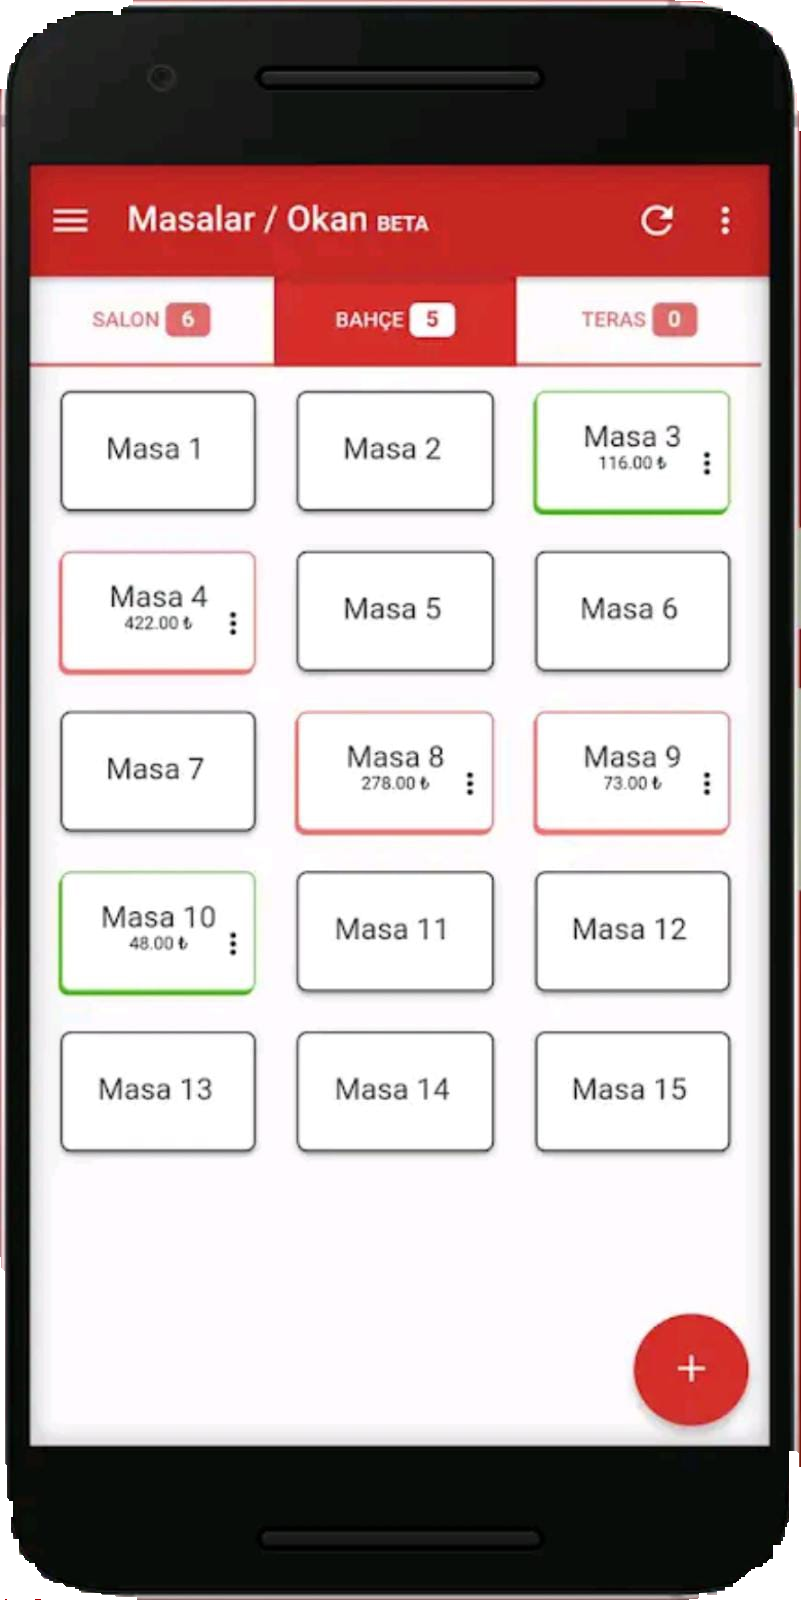
\includegraphics[width=5cm,height=6cm,keepaspectratio=true]{./fig/Adisyo-Masalar}
  \caption{Adisyo Personel'e ait ekran görüntüsü}
   \label{fig:ch2-1-1}
\end{figure}


\subsection{Qr kod menü}

Kafeye ait menünün fotoğrafını çekip uygulamaya yükleyeceğimiz ve bunun sonucunda bize bir QR kod oluşturacağı bir mobil uygulamadır. Bu QR kod sayesinde menüyü görebiliriz.
\begin{figure} [h]
 \centering
 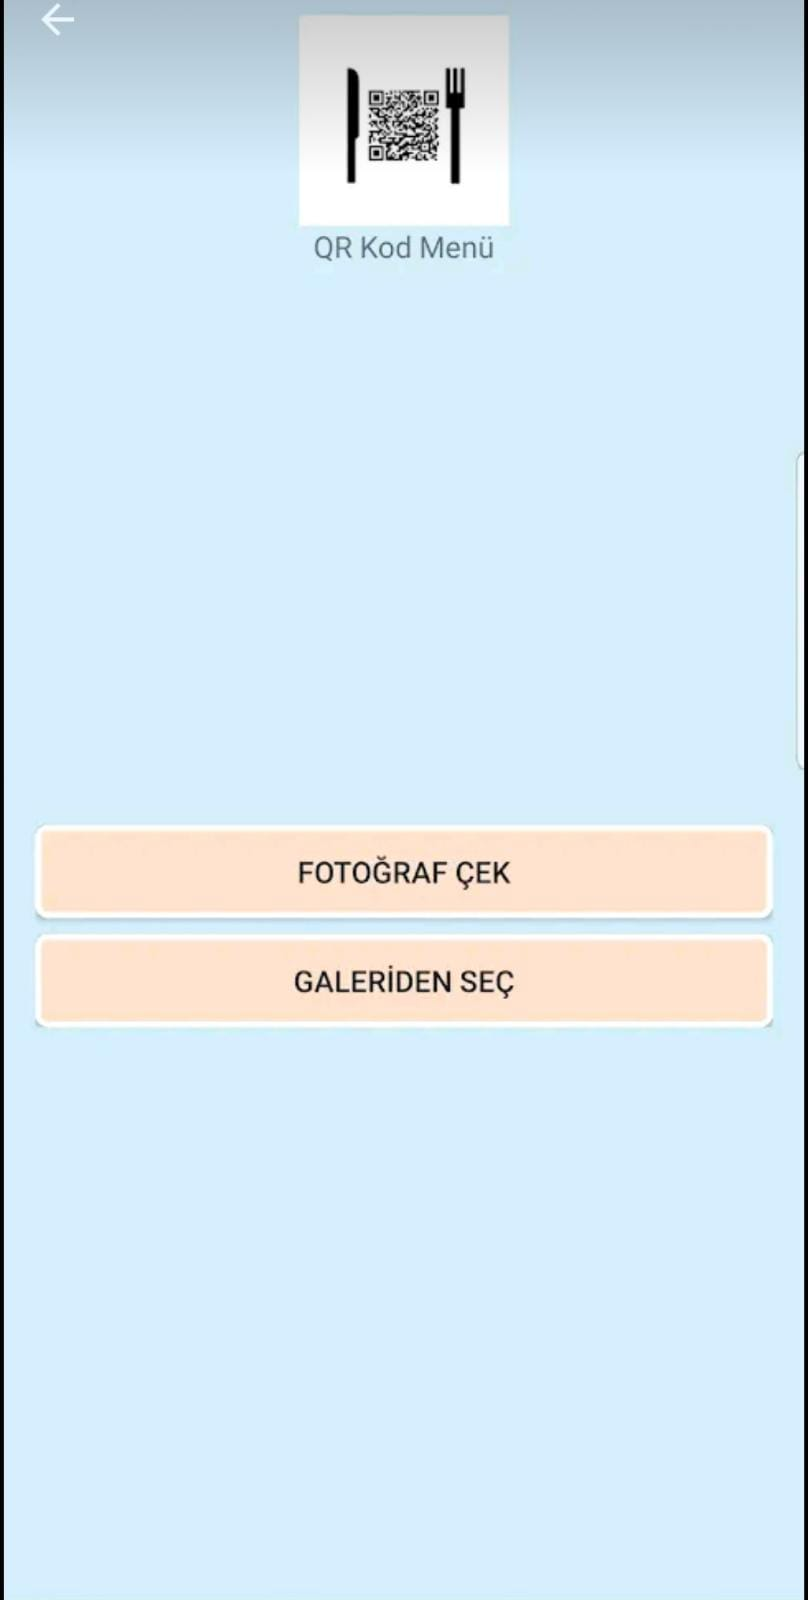
\includegraphics[width=5cm,height=6cm,keepaspectratio=true]{./fig/Qrkod-Menu}
  \caption{Qr kod menü'ye ait ekran görüntüsü}
 \label{fig:ch2-1-2}
\end{figure}

\section{Öğrenci İşleri Uygulaması}
Öğrenci İşleri'nin web uygulamasının bir kısmını kodladım. Bunun sonucunda ortaya çıkan görseller aşağıda gösterilmiştir.

\subsection{Bilgisayar ile web sitesine giriş}
Bilgisayardan menüye bakacak olursak eğer uygulamaya ait ekran görüntüsü aşağıda gösterilmiştir.
\begin{figure} [h]
 \centering
 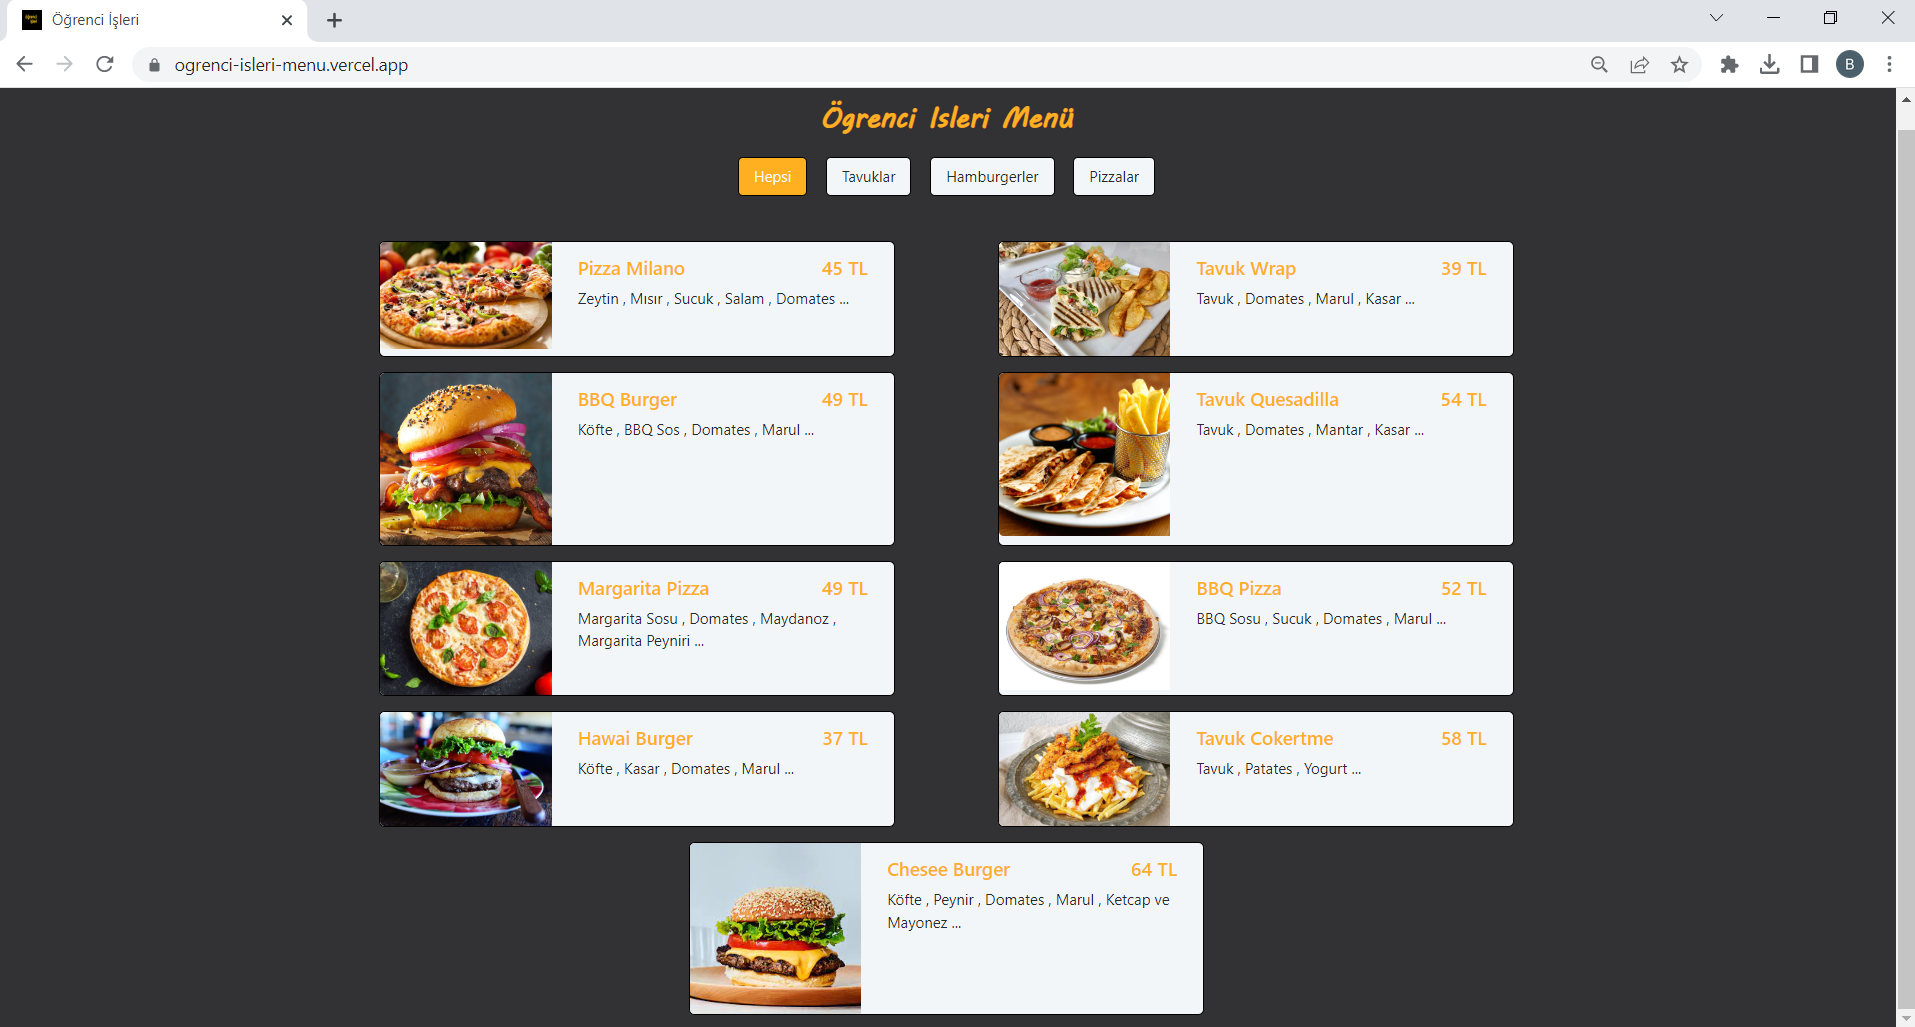
\includegraphics[width=380pt,keepaspectratio=true]{./fig/Ogrenci-Isleri}
  \caption{Öğrenci işleri'nin bilgisayar üzerinde menünün görüntüsü}
 \label{fig:ch2-2-1}
\end{figure}

\subsection{Mobil cihaz ile web sitesine giriş}
Uygulamanın web kısmını kodlarken responsive yapıda olmasına özen gösterdim. 
 (Örnek: {\bf Şekil: 2.4})
\begin{figure} [h]
 \centering
 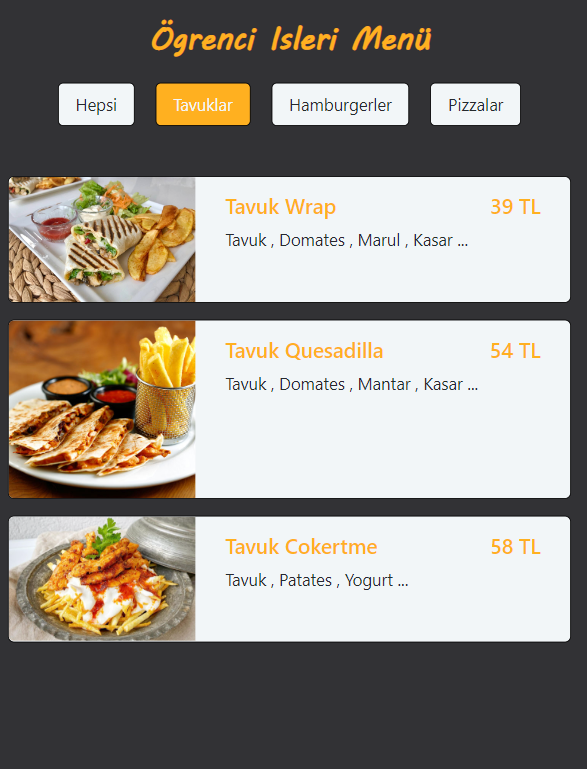
\includegraphics[width=5cm,height=10cm,keepaspectratio=true]{./fig/Ogrenci-Mobil}
  \caption{Öğrenci işleri'nin mobil cihaz üzerinde menünün görüntüsü}
 \label{fig:ch2-2-2}
\end{figure}






